\documentclass[footline=authortitle]{beamer}
\usepackage{graphicx} % Required for inserting images
\usepackage[dvipsnames]{xcolor}
\usepackage[english]{babel}
\usepackage{ragged2e}
\usepackage{hyphenat}
\usepackage{siunitx}

\usepackage{listings}
\usepackage{xcolor}
\usepackage{wrapfig}


\lstset{
  language=Python,
  basicstyle=\ttfamily\footnotesize,
  keywordstyle=\color{blue},
  commentstyle=\color{gray},
  stringstyle=\color{orange},
  showstringspaces=false,
  breaklines=true,
}

\usepackage{biblatex}
\addbibresource{bib.bib}

\mode<presentation>{
  \usetheme{Frankfurt}
  \usecolortheme[named=PineGreen]{structure}
  \useoutertheme{default} % solo UNA volta
  \setbeamertemplate{headline}{}  % rimuove del tutto la barra in alto

  \makeatletter
  \setbeamertemplate{footline}{
    \leavevmode%
    \hbox{%
      \begin{beamercolorbox}[wd=.65\paperwidth,ht=2.5ex,dp=1ex,center]{author in head/foot}%
        \usebeamerfont{author in head/foot}\insertshortauthor
      \end{beamercolorbox}%
      \begin{beamercolorbox}[wd=.1\paperwidth,ht=2.5ex,dp=1ex,center]{frame number in head/foot}%
        \insertframenumber{} / \inserttotalframenumber
      \end{beamercolorbox}%
      \begin{beamercolorbox}[wd=.25\paperwidth,ht=2.5ex,dp=1ex,center]{title in head/foot}%
        \usebeamerfont{title in head/foot}\insertshorttitle
      \end{beamercolorbox}%
    }
    \vskip0pt%
  }

  \setbeamercovered{transparent}
  \setbeamercolor{block title example}{fg=white,bg=Blue}
  \setbeamercolor{block body example}{fg=black,bg=Blue!10}
  \setbeamercolor{postit}{fg=black,bg=OliveGreen!20}
  \setbeamercolor{postit2}{fg=yellow,bg=OliveGreen}
}

\title[Computational Imaging]{Meteorological Super-Resolution\\vs\\Wind Representations}
\author[Gruppo 21 - Marzia De Maina, Matteo Galiazzo, Federica Santisi]
{Gruppo 21\\Marzia De Maina, Matteo Galiazzo, Federica Santisi}
\institute[Alma Mater Studiorum - Università di Bologna]
{
  \textit{Alma Mater Studiorum - Università di Bologna}\\[0.25Cm]
  \textit{Dipartimento di Informatica - Scienza e Ingegneria (DISI)} \\[0.5Cm]
  Prof. \textbf{Fabio Merizzi}\\
  }
\date{}
\begin{document}
\begin{frame}[fragile]
    \titlepage
    
\end{frame}

\begin{frame}{Purpose}
  \begin{itemize}
    \item \textbf{Objective:} Evaluate the impact of different wind representations on neural-based super-resolution for meteorological fields.
    \item Compare two wind encodings:
      \begin{itemize}
        \item Orthogonal components $u_{10},\,v_{10}$
        \item Polar form: speed and direction (degrees from north)
      \end{itemize}
    \item Use ERA5 (30 km) and VHR-REA (2.2 km) datasets for training and testing.
    \item Assess which representation yields better performance (MSE) and qualitative reconstruction.
  \end{itemize}
\end{frame}
% COSE DA AGGIUNGERE PER ROSICCHIARE TEMPO
% CONFIFGURAZIONE DELL'AMBIENTE, DOVE ABBIAMO FATTO IL TRAINING E COME ABBIAMO GESTITO IL TUTTO

% MARZIA
% Wind Field Representations
\begin{frame}{Wind Field Representations}
  \begin{columns}
    \column{0.47\textwidth}
      \textbf{Cartesian Components}\
      \begin{itemize}
        \item $u_{10}, v_{10}$: zonal and meridional wind at 10m height
        \item Directly match ERA5 outputs
      \end{itemize}
    \column{0.53\textwidth}
      \textbf{Polar Encoding}\
      \begin{itemize}
        \item $\text{speed}=\sqrt{u_{10}^2 + v_{10}^2}$
        \item $\text{direction}=(180 + \frac{180}{\pi}\arctan2(-u_{10}, -v_{10}))\bmod360$
      \end{itemize}
  \end{columns}
  \vspace{1cm}
  \textbf{Motivation:} Representation may affect neural network learning and reconstruction quality. \cite{merizzi}
\end{frame}
% riprendere la consegna ricordando che consegna avevamo, cosa era richiesto e fare una panoramica sulla teoria necessaria (unet)

%%%%% Super-Resolution and U-Net Theory
\begin{frame}{Super-Resolution and U-Net Theory}
  \begin{itemize}
    \item \textbf{Super-Resolution:} Upscaling low-resolution fields to high-resolution targets using deep learning. %\cite{SR_meteorology2024}.
    \vspace{0.5cm}
    \item \textbf{U-Net Architecture:} Encoder–decoder with skip connections for image-to-image tasks \cite{ronneberger2015u}.
      \begin{itemize}
        \item Residual blocks to ease training.
        \item Multiscale features preserved via concatenation.
      \end{itemize}
      \vspace{0.5cm}
    \item \textbf{Metrics:} Mean Squared Error (MSE) on test set.
  \end{itemize}
\end{frame}

% FEDE
\begin{frame}{Datasets and Preprocessing}
% parlare dei 2 dataset (all'inizio erano 3) + come li abbiamo gestiti (preprocessing + abbiamo ritagliato per salvare risorse + minmax normalizzatione)
% parlare del datset di train locale piccolo da 100 esempi per esperimenti e quello su colab da 1000 esempi per training effettivo
\end{frame}

\begin{frame}{Datasets and Preprocessing}
    For the purpose of this project, the wind field representations are derived from the ERA5 and VHR--REA datasets.
    \vspace{1em}
        \begin{itemize}
            \item \textbf{ERA5} is a global reanalysis dataset developed by ECMWF, providing hourly data since 1950 at a 0.25° (\textasciitilde31 km) resolution.
            \item \textbf{VHR--REA} is a downscaled regional reanalysis for Italy based on the COSMO model, with a resolution of 2.2 km.
        \end{itemize}
    \vspace{1em}
    Both datasets are aligned temporally (06, 12, 18, 00 UTC) and spatially through reprojection. \\
    \vspace{1em}
    ERA5 acts as the low-resolution input; VHR--REA is used as the high-resolution target for training.
\end{frame}

\begin{frame}{Datasets and Preprocessing}
\scriptsize
    \begin{columns}
        \begin{column}{0.65\textwidth}
            \begin{itemize}
                \item \textbf{ERA5} is the fifth-generation global reanalysis dataset produced by ECMWF under the Copernicus Climate Change Service (C3S). 
                It replaces the previous ERA-Interim product, offering higher accuracy, finer temporal and spatial resolution (0.25°), and consistent uncertainty estimates.

                \vspace{0.8em}
            
                \item Based on a 4D-Var data assimilation scheme, ERA5 integrates a vast range of observational data, including satellite, radiosonde, buoy, and aircraft measurements. 
                It covers the atmosphere, land surface, and ocean waves with hourly updates and is widely used for climate studies, energy forecasting, and risk assessment.

                \vspace{0.8em}

                \item In this project, we focus on the surface wind fields, specifically the \texttt{u10} and \texttt{v10} components, which serve as low-resolution inputs for the super-resolution model.
            \end{itemize}
        \end{column}

        \begin{column}{0.35\textwidth}
            \centering
            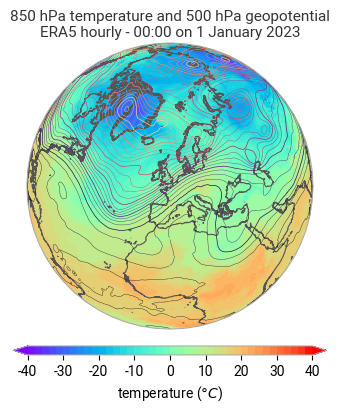
\includegraphics[width=\linewidth]{images/overview-detail_67e6d1d5ac470ee33ae510a76a2fe3c1c67a7f1fdd4c040a333969fe0b11f76f.png}
        \end{column}
    \end{columns}

\end{frame}

\begin{frame}{Datasets and Preprocessing}
    \begin{wrapfigure}{r}{0.4\textwidth}
        \centering
        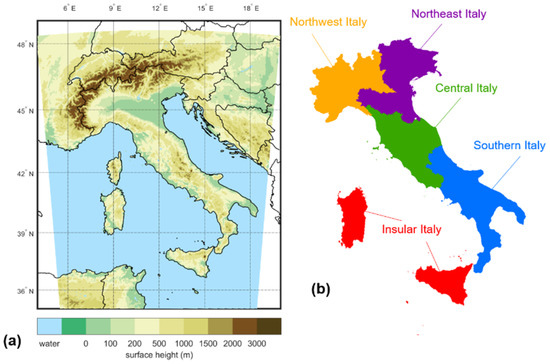
\includegraphics[width=0.38\textwidth]{images/data-06-00088-g001-550.jpg}
        \caption*{\tiny VHR--REA spatial coverage over Northern Italy}
    \end{wrapfigure}
    \scriptsize
    \textbf{VHR--REA (Very High Resolution ReAnalysis)} is a dataset produced by CMCC by dynamically downscaling ERA5 with the COSMO regional model. The dataset has ~2.2 km resolution, explicitly resolving convection processes important in complex terrain.

    This high-resolution data supports regional applications such as hydrological forecasting, renewable energy planning, and urban climatology.

    \begin{itemize}
        \item Target resolution for training a super-resolution model.
        \item Data span: one full year, 4 times daily over Northern Italy.
    \end{itemize}
\end{frame}


\begin{frame}[fragile]
\frametitle{Dataset and Preprocessing}
\scriptsize
\begin{columns}
    % Colonna sinistra: testo
    \begin{column}{0.55\textwidth}
        \textbf{Spatial Alignment \& Patch Extraction}
        \begin{itemize}
            \item Center crop to 224×224 pixel patches
            \item Temporal synchronization verification
            \item Channel-wise data stacking (u10, v10 components)
            \item Custom PyTorch Dataset implementation
        \end{itemize}

        \textbf{Data Pipeline Architecture}
        \begin{itemize}
            \item ItalyWeatherDataset class for paired data loading
            \item Automatic temporal alignment checking
            \item Flexible normalizer integration
            \item Memory-efficient batch processing
        \end{itemize}

        \textbf{Quality Assurance}
        \begin{itemize}
            \item Index bounds verification
            \item Consistent tensor dimensions
            \item Error handling for misaligned datasets
        \end{itemize}
    \end{column}

    % Colonna destra: codice
    \begin{column}{0.45\textwidth}
        \begin{lstlisting}[language=Python, basicstyle=\ttfamily\tiny]
def extract_region(self, data_tensor):
    patch_h, patch_w = (224, 224)
    _, h, w = data_tensor.shape
    x = (w - patch_w) // 2
    y = (h - patch_h) // 2
    return data_tensor[:, 
                      y:y+patch_h, 
                      x:x+patch_w]

def __getitem__(self, idx):
    era_slice = self.era5_dataset.isel(valid_time=idx)
    era_arrays = [era_slice[v].values 
                  for v in self.ERA5_VARIABLES]
    era_tensor = torch.from_numpy(
        np.stack(era_arrays, axis=0)).float()
    era_tensor = self.extract_region(era_tensor)

    if self.era5_normalizer:
        era_tensor = self.era5_normalizer.normalize(era_tensor)
        \end{lstlisting}
    \end{column}
\end{columns}
\end{frame}


\begin{frame}[fragile]
\frametitle{Normalization \& Coordinate Transformation}
\tiny
\begin{columns}
\begin{column}{0.4\textwidth}
\textbf{MinMax Normalization Strategy}
\begin{itemize}
    \item Training-based statistics computation
    \item Per-channel normalization across spatial dimensions
    \item Feature range scaling to [0, 1]
    \item Epsilon handling for division-by-zero cases
    \item Serializable normalizer objects
\end{itemize}

\vspace{0.3cm}

\textbf{Coordinate System Transformation}
\begin{itemize}
    \item \textbf{Option 1}: Cartesian coordinates (u, v)
    \item \textbf{Option 2}: Polar coordinates (magnitude, direction)
    \item $magnitude = \sqrt{u^2 + v^2}$
    \item $direction = 180° + \frac{180°}{\pi} \arctan2(-u, -v) \bmod 360°$
\end{itemize}

\vspace{0.3cm}

\textbf{Dataset Management}
\begin{itemize}
    \item 80-20 train-test split with fixed seed (42)
    \item Separate normalization preservation
    \item Batch processing with memory optimization
\end{itemize}
\end{column}

\begin{column}{0.6\textwidth}

\begin{lstlisting}[language=Python, basicstyle=\ttfamily\tiny]
class MinMaxNormalizer:
    def compute_stats(self, data_tensor):
        # Min/max per channel across (N,H,W) dims
        self.min_val = data_tensor.amin(
            dim=(0, 2, 3), keepdim=True)
        self.max_val = data_tensor.amax(
            dim=(0, 2, 3), keepdim=True)
        
        # Handle division by zero
        diff = self.max_val - self.min_val
        epsilon = 1e-7
        self.max_val[diff < epsilon] = \
            self.min_val[diff < epsilon] + epsilon
    def normalize(self, x):
        return (x - self.min_val) / \
               (self.max_val - self.min_val)

# Coordinate transformation to polar
if COORDINATES == "1":
    u_squared = tensor[0, :, :]**2
    v_squared = tensor[1, :, :]**2
    magnitude = torch.sqrt(u_squared + v_squared)
    direction = (180 + (180/math.pi) * 
                torch.atan2(-u_squared, -v_squared)) % 360
    tensor = torch.stack([magnitude, direction], axis=0)
\end{lstlisting}
\end{column}
\end{columns}

\end{frame}



% --- MATTEO ---
% spiegare che modello abbiamo usato (upconv vs bilinear upsampling) + come abbiamo scelto la loss + come abbiamo scelto gli iperparametri
% [x] panoramica generale sul modello
% [x] upconv vs bilinear upsampling
% [x] loss
% [x] iperparametri (tabella)
\begin{frame}{Model and hyperparameters - Introduction}
\footnotesize
    Our model is based on the U-Net architecture, extended with residual connections for better gradient flow and stability.
    The input has 2 channels $(u,v)$ and the output also has the same 2 channels representing the high-resolution version of the same fields.

    The key building blocks are:
    \begin{itemize}
        \item \textbf{Residual Block}: it's the core module of the architecture. It has two paths
        \begin{itemize}
            \item One that applies convolutions and normalization.
            \item One that does nothing (the residual application).
        \end{itemize}
        The model learns how much to use either path.
        \item \textbf{Downsampling Block}: reduces the spatial resolution and increases the feature size. It uses stride 2 to downsample and includes a residual block.
        \item \textbf{Upsampling Block}: these are the mirror of down blocks. They use bilinear upsampling to increase the spatial dimension instead of transposed convolutions. Then, we concatenate  the skip connections from the encoder and use a $1\times 1$ convolution to reduce the number of channels after concatenations.
    \end{itemize}
    \end{frame}

    \begin{frame}{Model and hyperparameters}
    \centering
    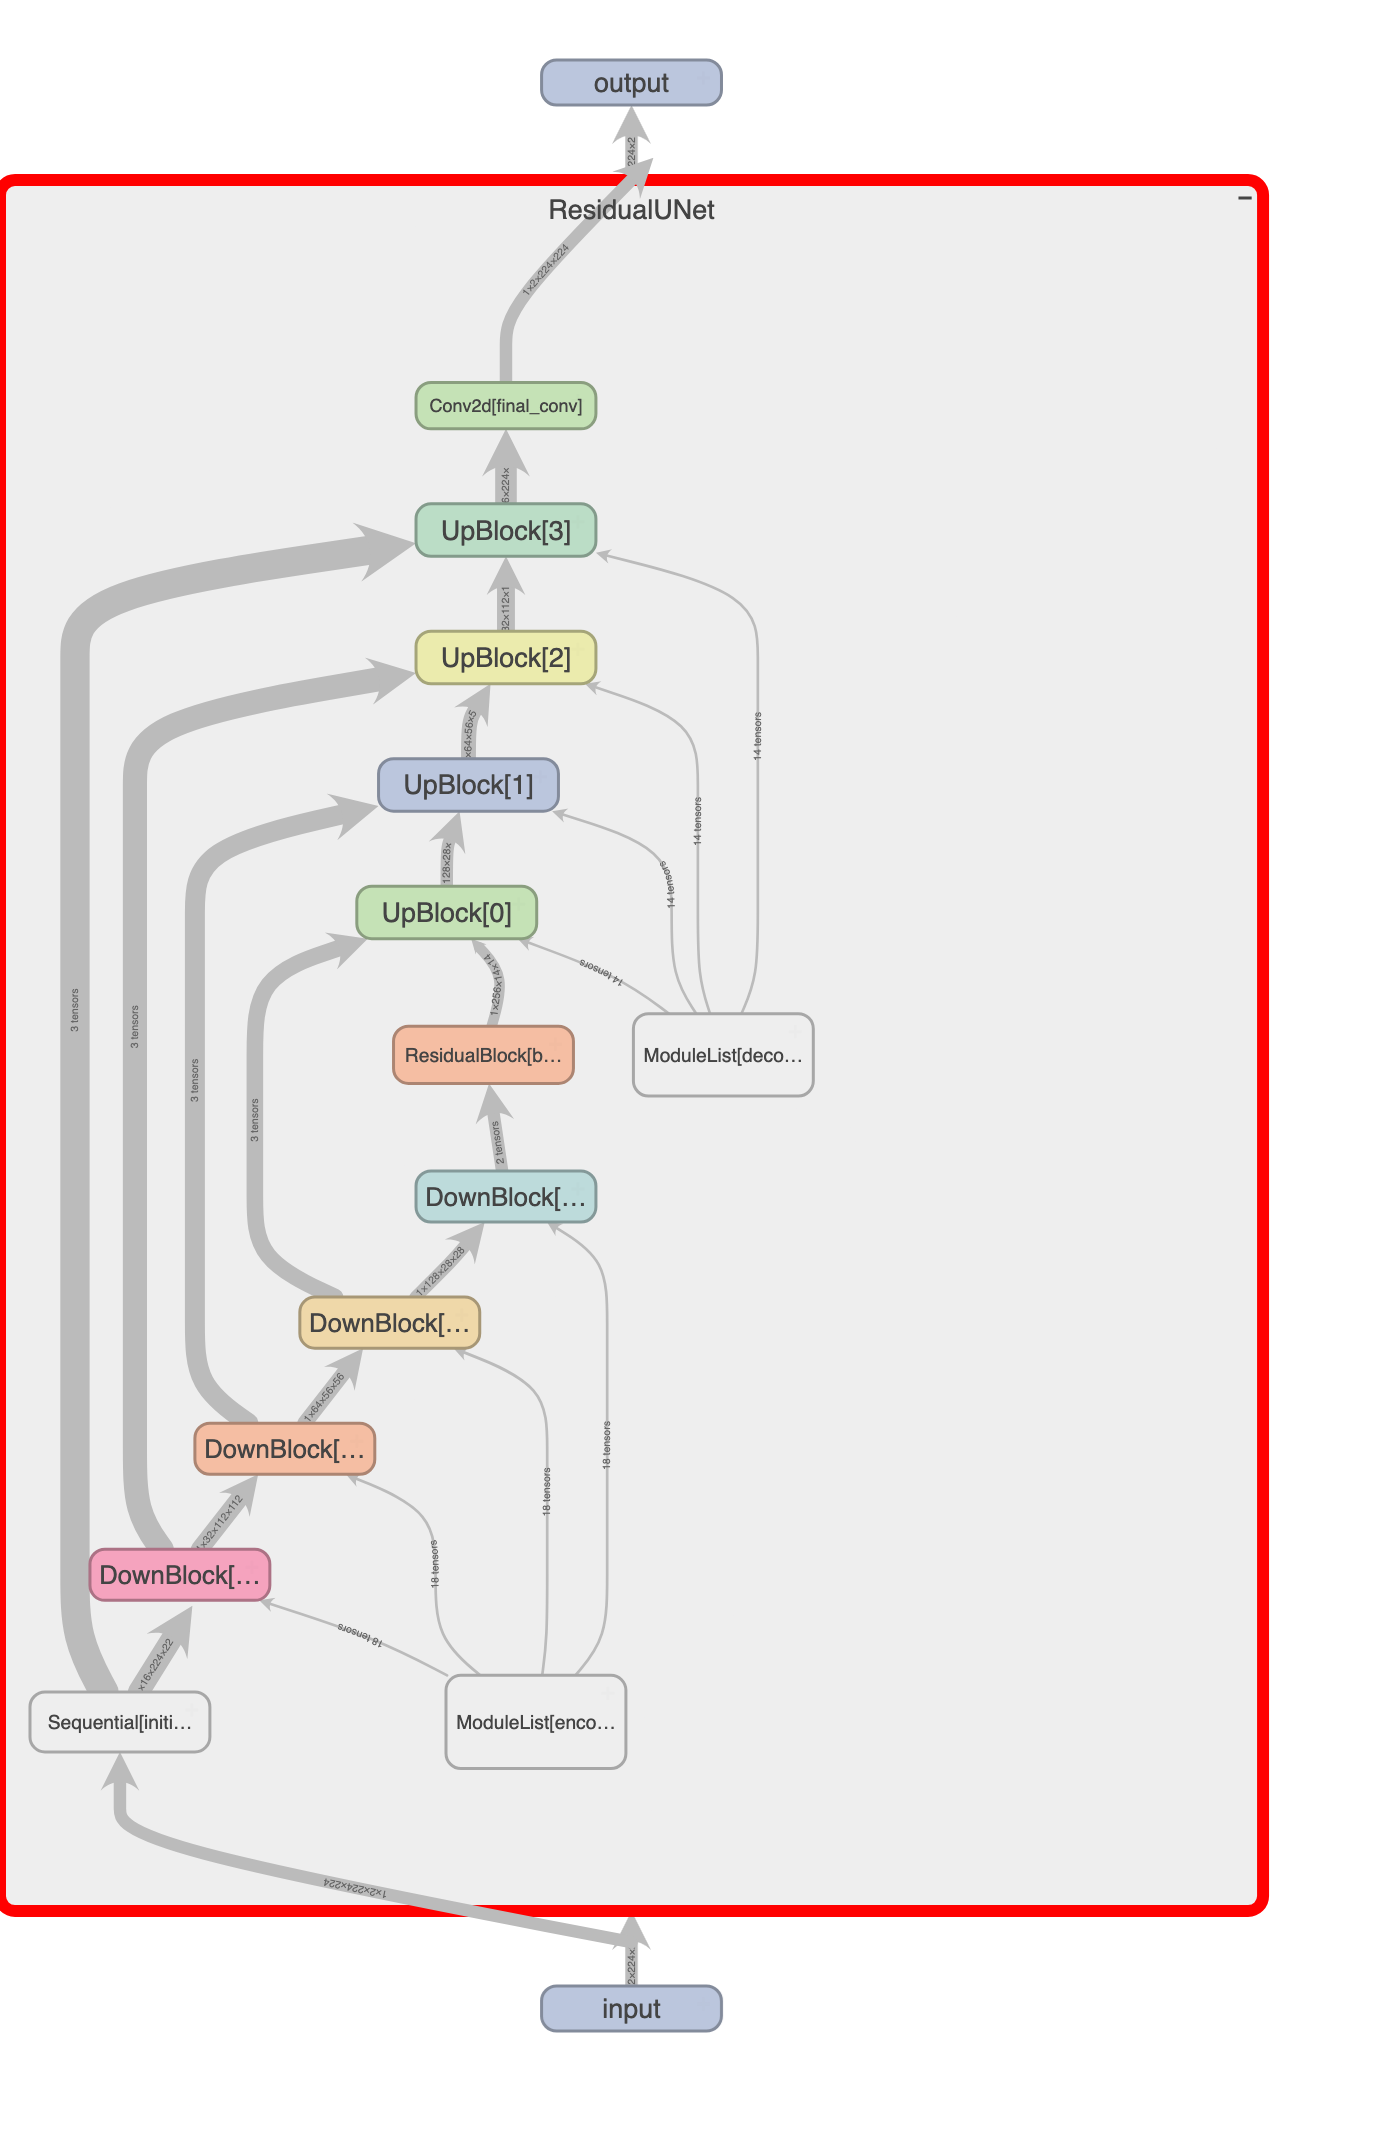
\includegraphics[width=0.45\textwidth]{images/unet_experiment_graph.png}
\end{frame}

\begin{frame}{Model and hyperparameters - Transposed vs Bilinear}

    \begin{table}[ht]
        \centering
        \scriptsize
        \begin{tabular}{|l|l|l|l|l|}
        \hline
        \textbf{Network Type} & \textbf{Parameters Count} & \textbf{Training Time} & \textbf{Test Loss} & \textbf{Test SSIM} \\
        \hline
        Transposed Conv & 13,041,922 (13.0 M) & 54:03 16.22s/it & 0.197755 & 0.709096 \\
        Bilinear Interp & 3,607,586 (3.6 M) & 08:04 2.42s/it & 0.171656 & 0.749828 \\
        \hline
        \end{tabular}
        \caption{Comparison of bilinear interpolation vs transposed convolution.}
        \label{tab:network_comparison}
    \end{table}
\end{frame}

\begin{frame}{Model and hyperparameters - Loss}
    Even the best model couldn't get decent results with the suggested MSE loss, so we adopted a combined loss approach
    \begin{columns}
        \column{0.5\textwidth}
            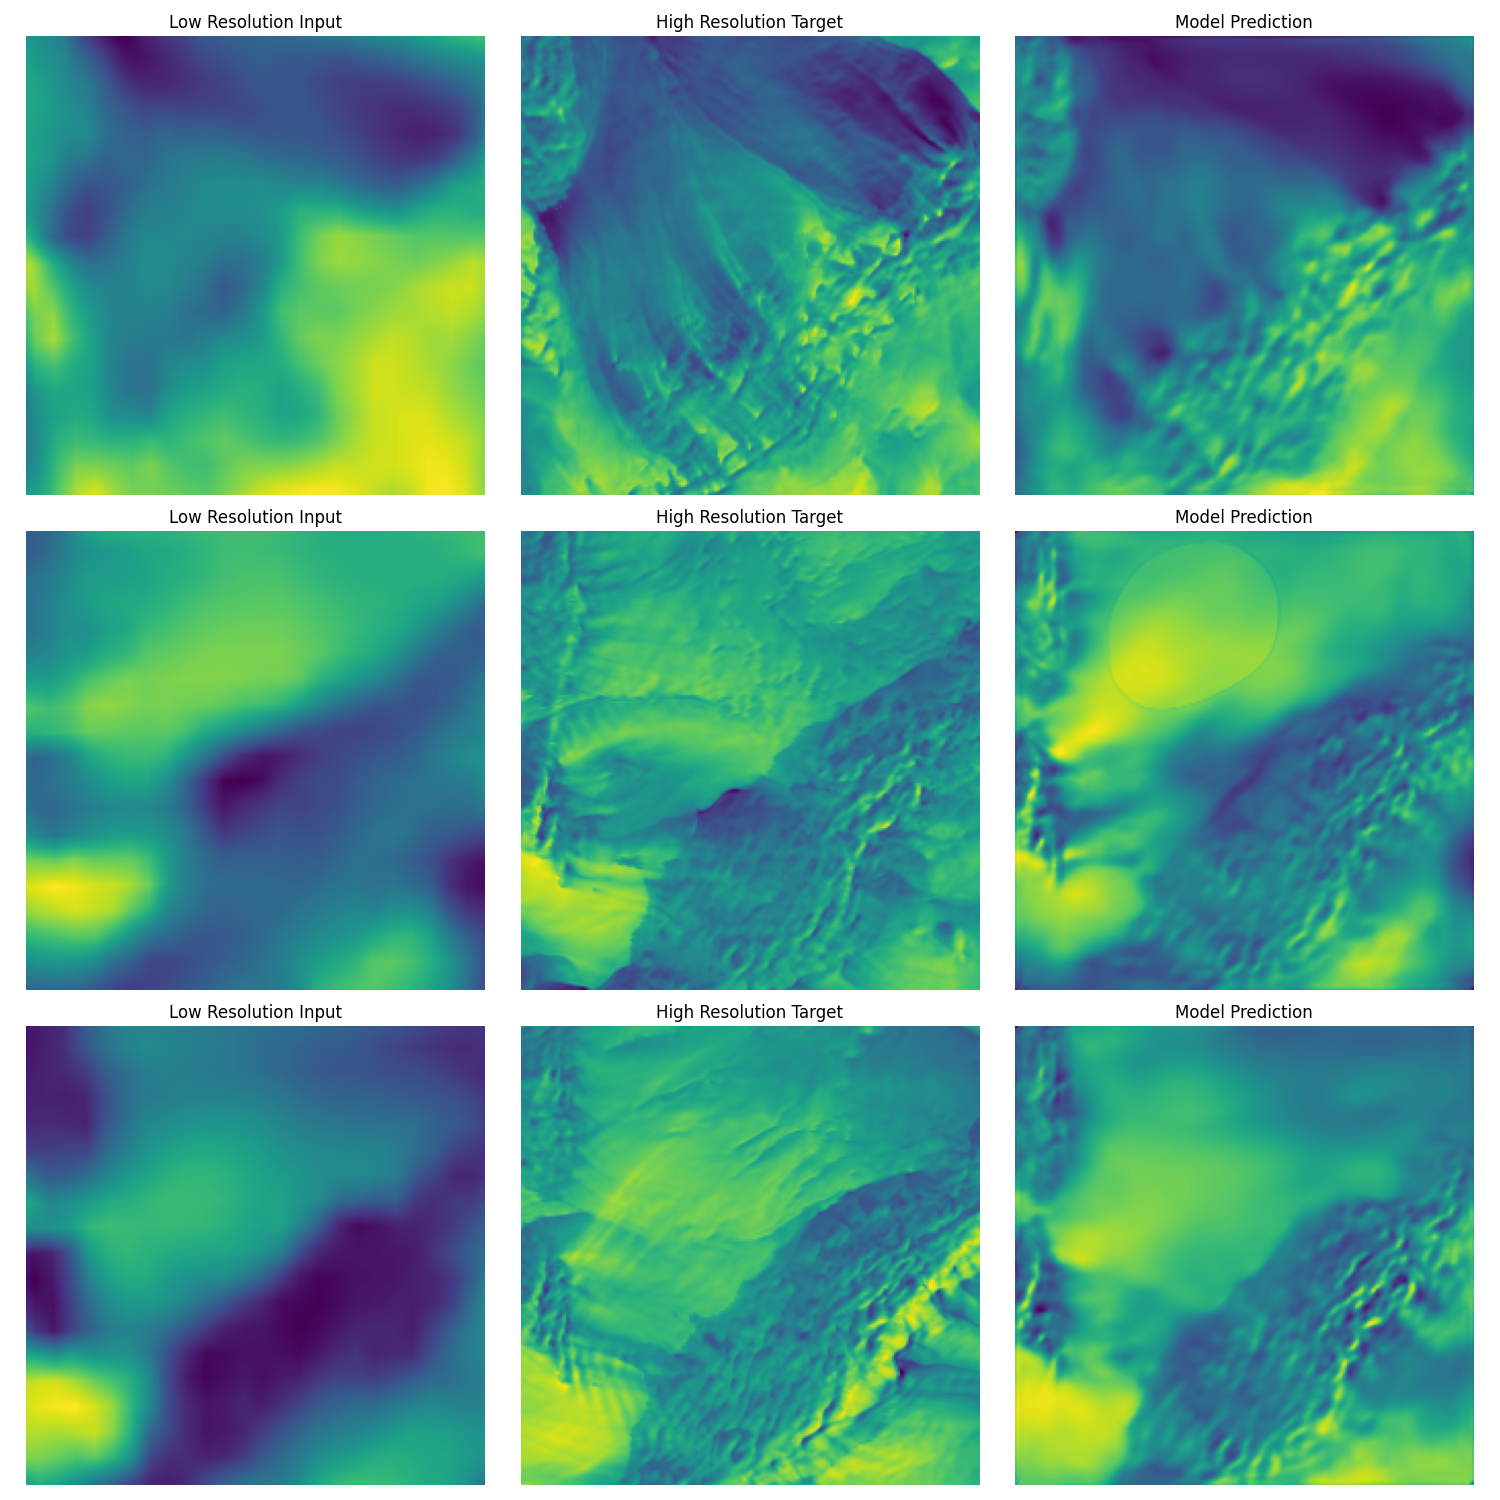
\includegraphics[width=\linewidth]{images/unet_vectors_l1ssim_loss_200_epochs_4_batch_1em3_lr_1em5_weightdecay.png}
            \newline
            \centering \small L1 + SSIM loss. SSIM: \texttt{0.7556}
        \column{0.5\textwidth}
            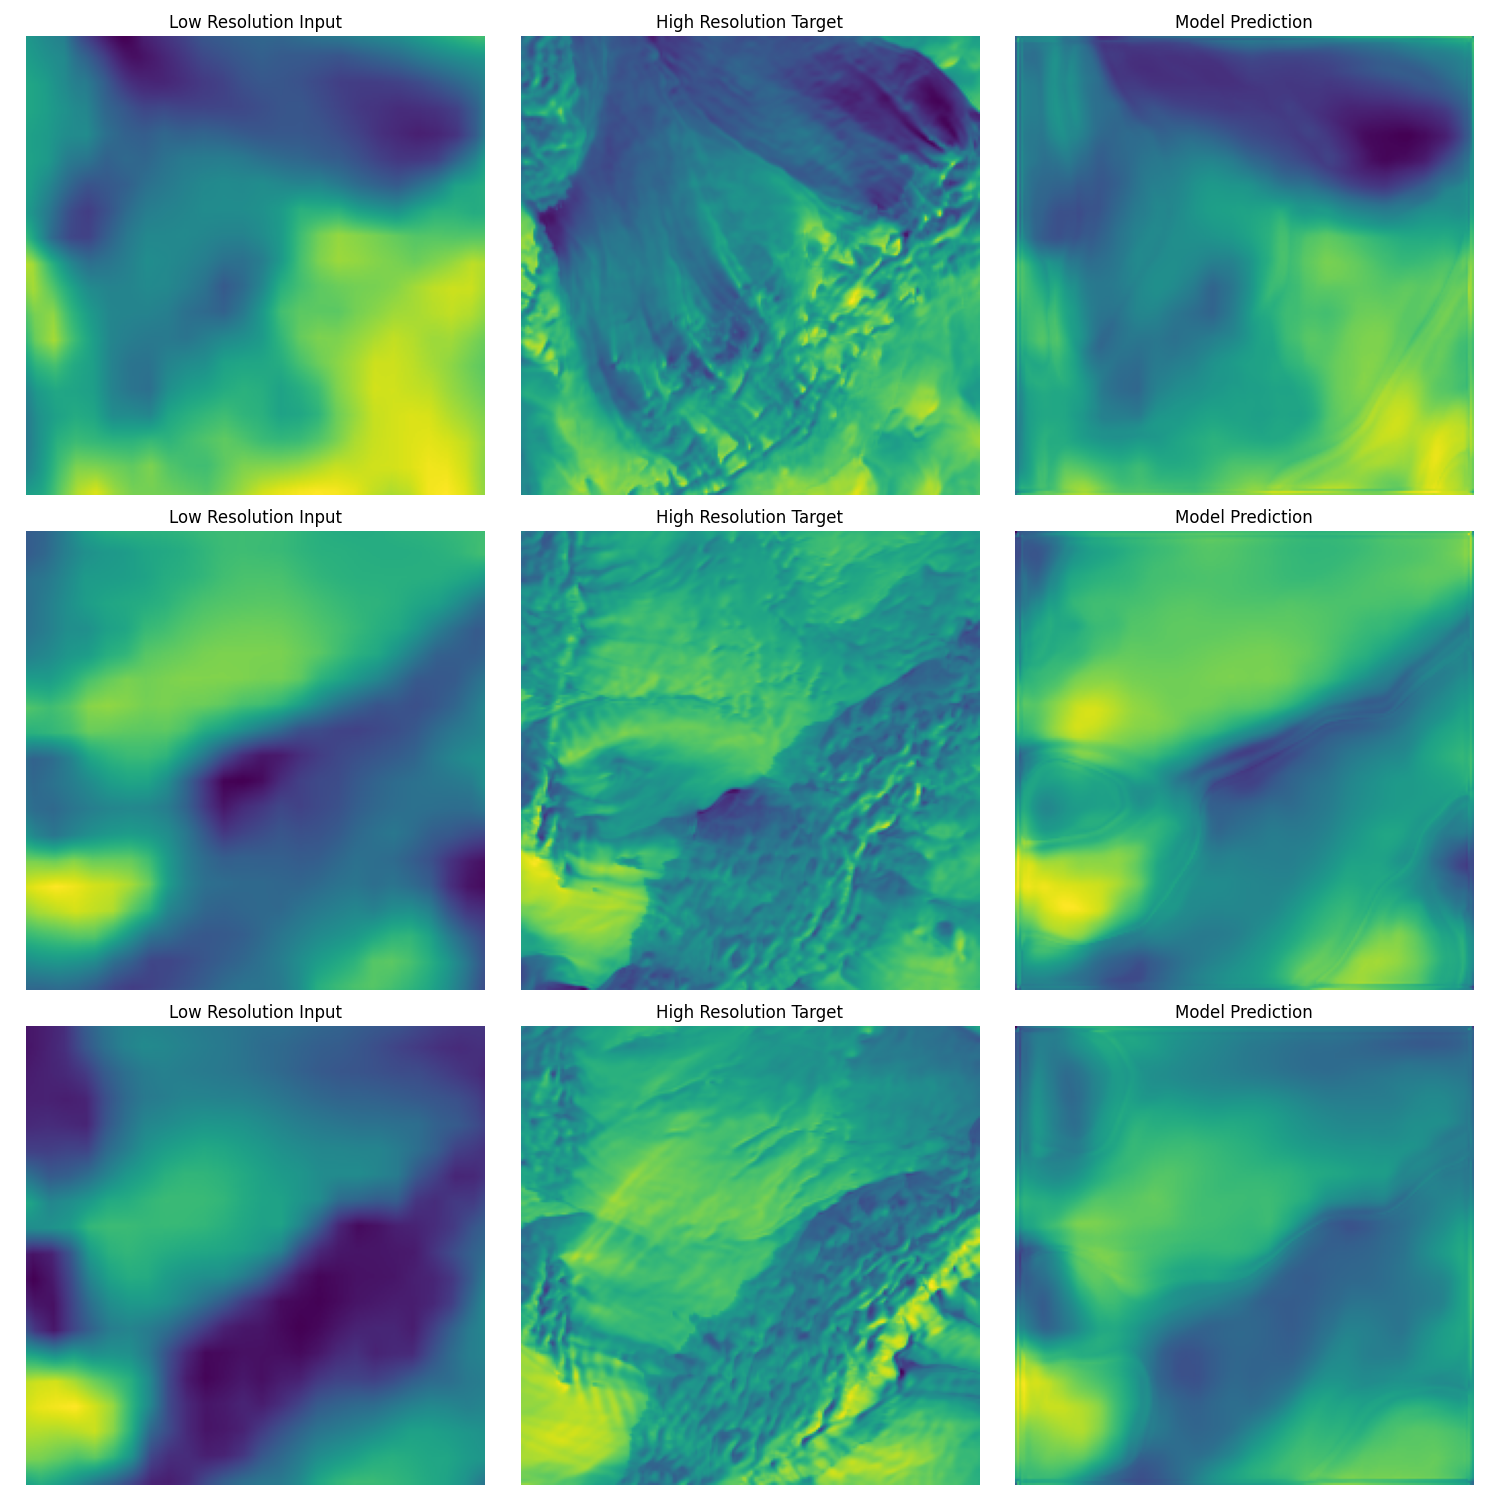
\includegraphics[width=\linewidth]{images/unet_vectors_mse_loss_200_epochs_4_batch_1em3_lr_1em5_weightdecay.png}
            \newline
            \centering \small MSE loss. SSIM: \texttt{0.7022}
    \end{columns}
\end{frame}

\begin{frame}[fragile]{Model and hyperparameters - Loss}
    \begin{lstlisting}
    class L1SSIMLoss(nn.Module):
    def __init__(self, alpha=0.85, ssim_window_size=11, ssim_data_range=1.0, ssim_channel=1):
        super(L1SSIMLoss, self).__init__()
        self.alpha = alpha
        self.l1_loss = nn.L1Loss() # Mean Absolute Error
        self.ssim_loss_fn = SSIMLoss(window_size=ssim_window_size, data_range=ssim_data_range, channel=ssim_channel)

    def forward(self, y_pred, y_true):
        ssim_val_loss = self.ssim_loss_fn(y_pred, y_true)
        l1_val_loss = self.l1_loss(y_pred, y_true)
        
        combined_loss = self.alpha * ssim_val_loss + (1 - self.alpha) * l1_val_loss
        return combined_loss
    \end{lstlisting}
\end{frame}

\begin{frame}{Model and hyperparameters - Hyperparameters}
    \begin{table}[ht]
        \centering
        \normalsize
        \resizebox{\textwidth}{!}{%
        \begin{tabular}{|c|c|c|c|c|c|c|c|c|}
        \hline
        \textbf{Channels} & \textbf{Epochs} & \textbf{Loss} & \textbf{Batch Size} & \textbf{LR} & \textbf{LR Scheduler} & \textbf{Weight Decay} & \textbf{Test Loss} & \textbf{Test SSIM} \\
        \hline
        {[}32, 64, 128{]} & 200 & L1 + SSIM & 8 & 1.00E-03 & NO & 1.00E-05 & 0.19090 & 0.71990 \\
        {[}16, 32, 64, 128{]} & 200 & L1 + SSIM & 8 & 1.00E-03 & NO & 1.00E-05 & 0.17700 & 0.74170 \\
        {[}16, 32, 64, 128, 256{]} & 300 & L1 + SSIM & 8 & 1.00E-03 & NO & 1.00E-05 & \textbf{0.16768} & \textbf{0.75555} \\
        {[}16, 32, 64, 128, 256{]} & 300 & MSE + SSIM & 8 & 1.00E-03 & NO & 1.00E-05 & \underline{0.15464} & \underline{0.75391} \\
        {[}16, 32, 64, 128, 256{]} & 300 & MSE & 8 & 1.00E-03 & NO & 1.00E-05 & 0.39491 & 0.52290 \\
        {[}16, 32, 64, 128, 256, 512{]} & 300 & L1 + SSIM & 8 & 1.00E-03 & NO & 1.00E-05 & 0.19207 & 0.71774 \\
        {[}16, 32, 64, 128, 256, 512{]} & 300 & L1 + SSIM & 8 & 1.00E-03 & YES & 1.00E-05 & 0.19207 & 0.71774 \\
        \hline
        \end{tabular}
        }
        \caption{Performance comparison of different network configurations. Best and runner-up models are highlighted in bold and underline, respectively.}
    \end{table}
\end{frame}

% --- MATTEO ---
% [x] curve di training
\begin{frame}[fragile]{Local Training - Loss and SSIM curves}
    Training curves for the best model on local data (loss and SSIM):
    \newline
    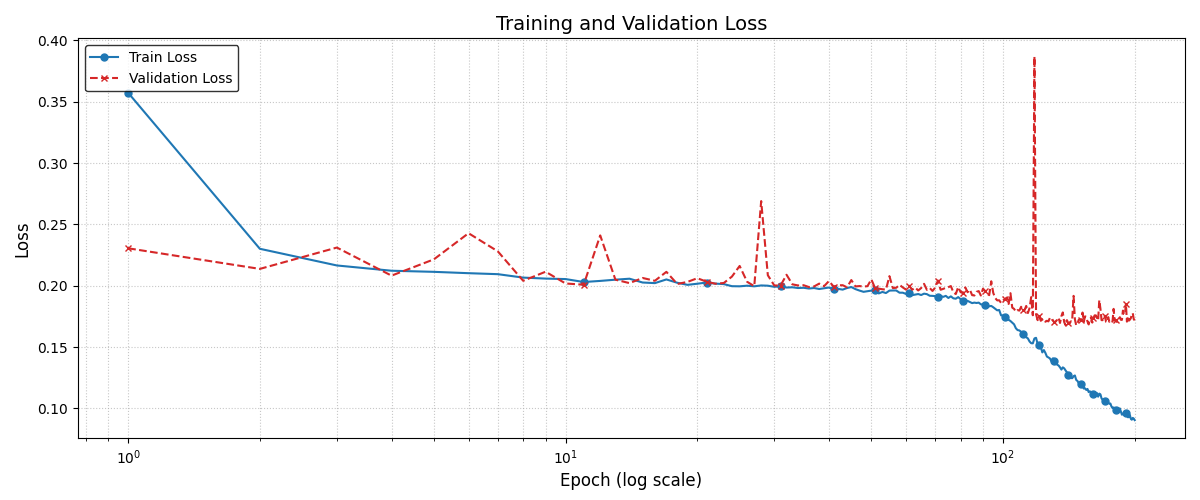
\includegraphics[width=0.7\linewidth]{images/local_loss_curve.png}
    \newline
    \small Loss curve 
    \newline
    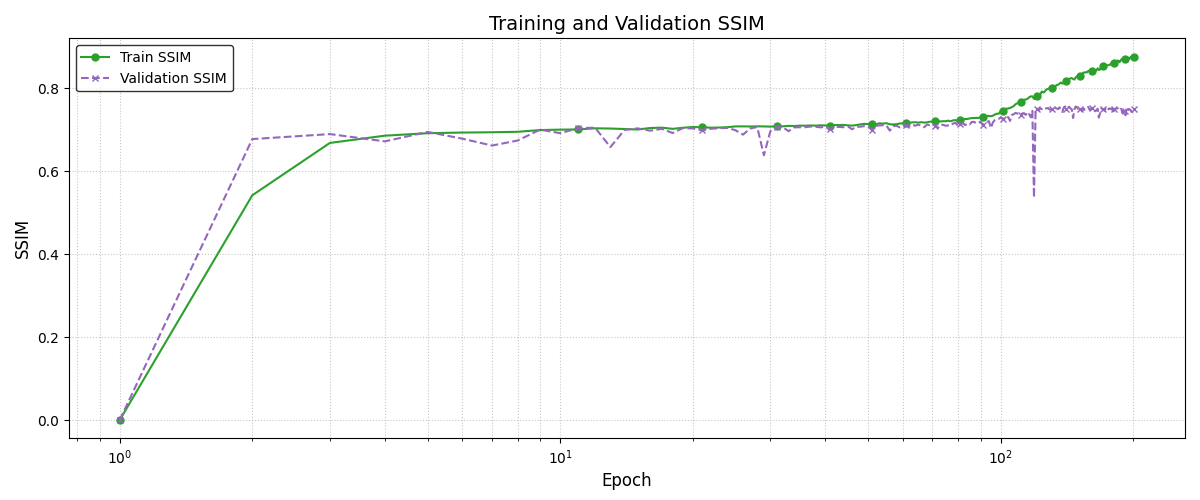
\includegraphics[width=0.7\linewidth]{images/local_ssim_curve.png}
    \newline
    \small SSIM curve 
\end{frame}

\begin{frame}{Colab Training - Difference with Local data}
    \begin{columns}
        \column{0.5\textwidth}
            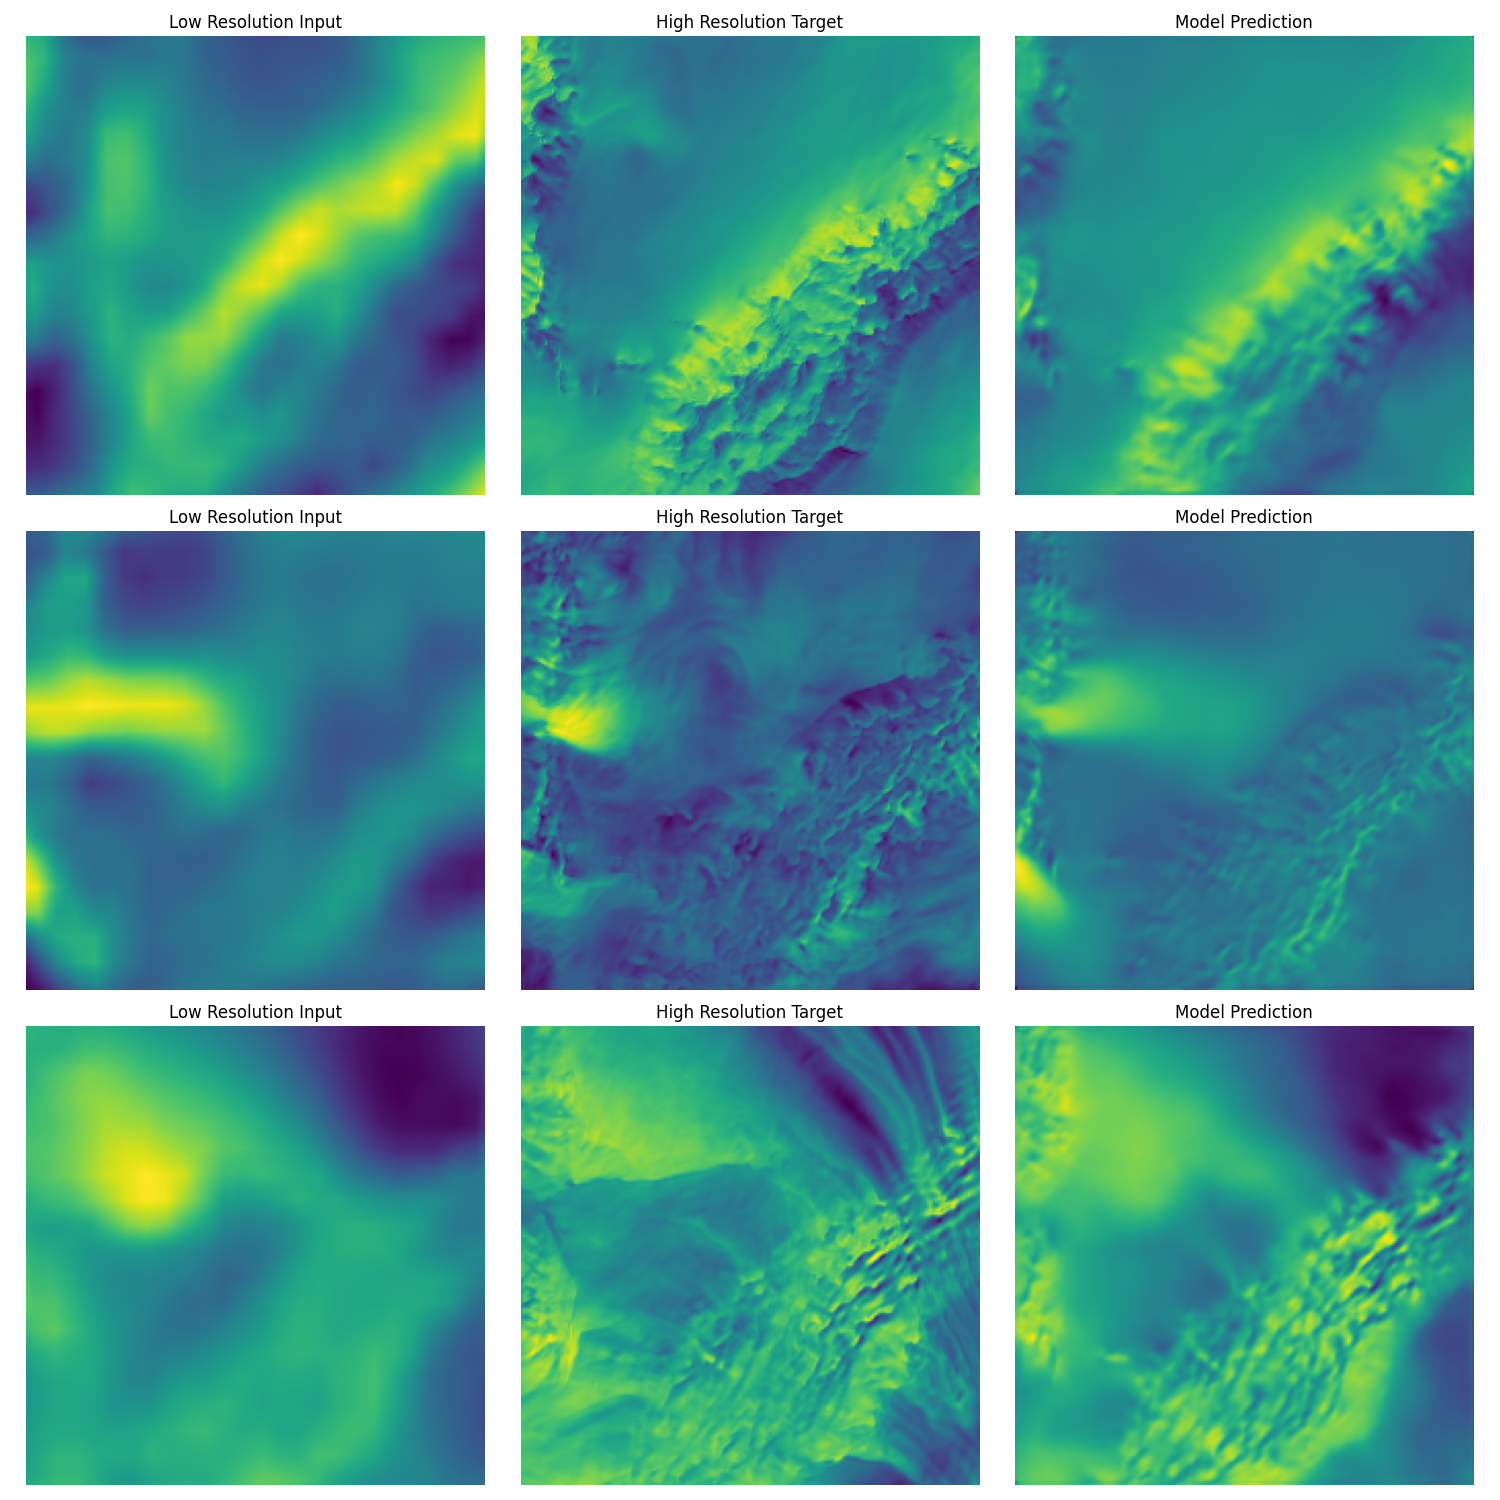
\includegraphics[width=\linewidth]{images/colab_vector_unet_L1SSIM_loss_300_epochs_8_batch_1em3_lr_1em5_weightdecay_best.pt.png}
            \newline
            \centering \small Colab data. SSIM: \texttt{0.84483}
        \column{0.5\textwidth}
            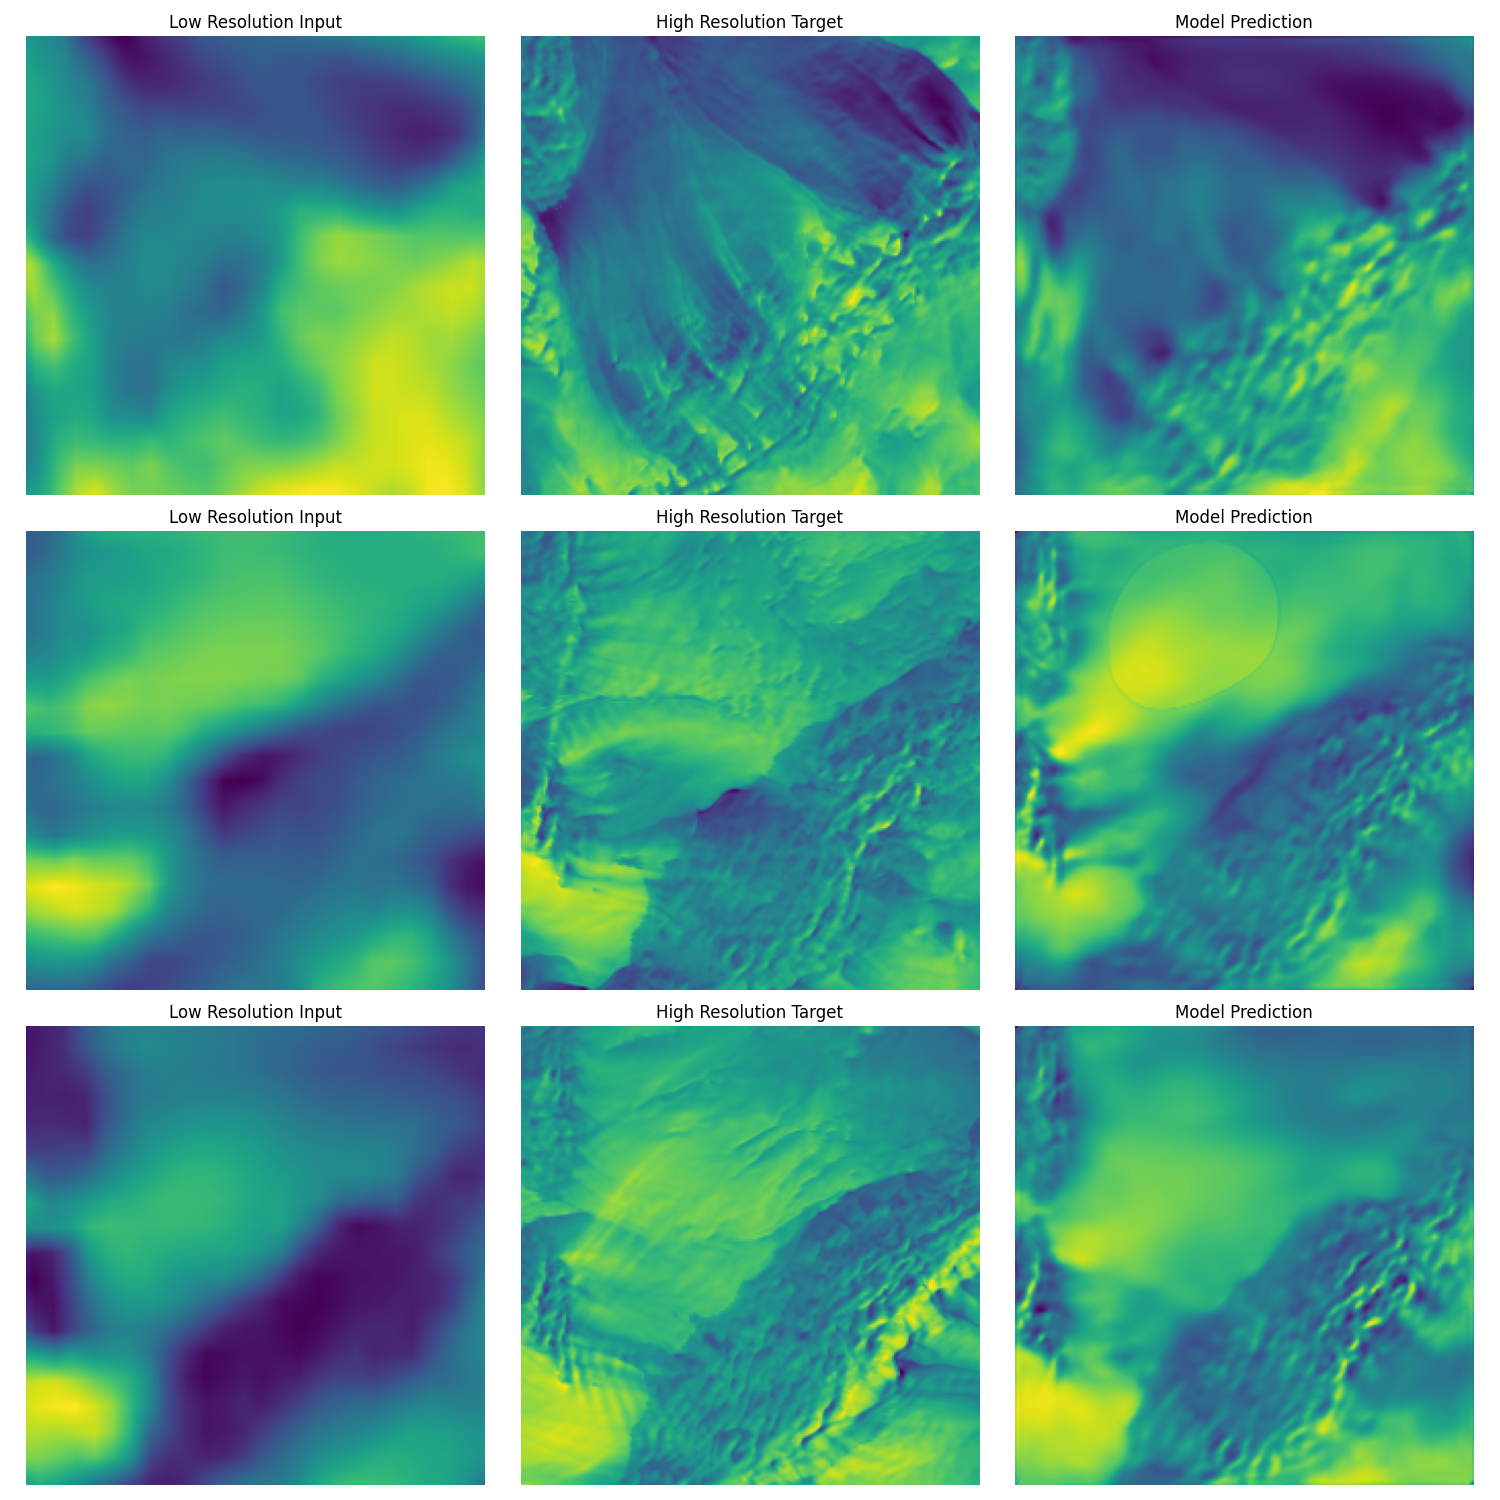
\includegraphics[width=\linewidth]{images/unet_vectors_l1ssim_loss_200_epochs_4_batch_1em3_lr_1em5_weightdecay.png}
            \newline
            \centering \small Local data. SSIM: \texttt{0.7556}
    \end{columns}
\end{frame}

\begin{frame}[fragile]{Colab Training - Loss and SSIM curves}
    Training curves for the best model on colab data (loss and SSIM):
    \newline
    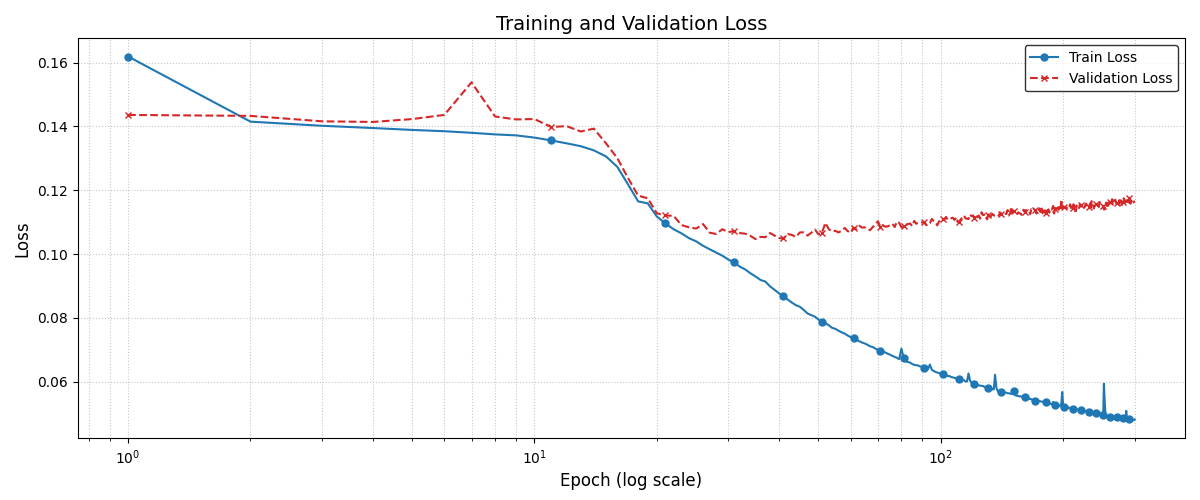
\includegraphics[width=0.7\linewidth]{images/colab_loss_curve.png}
    \newline
    \small Loss curve 
    \newline
    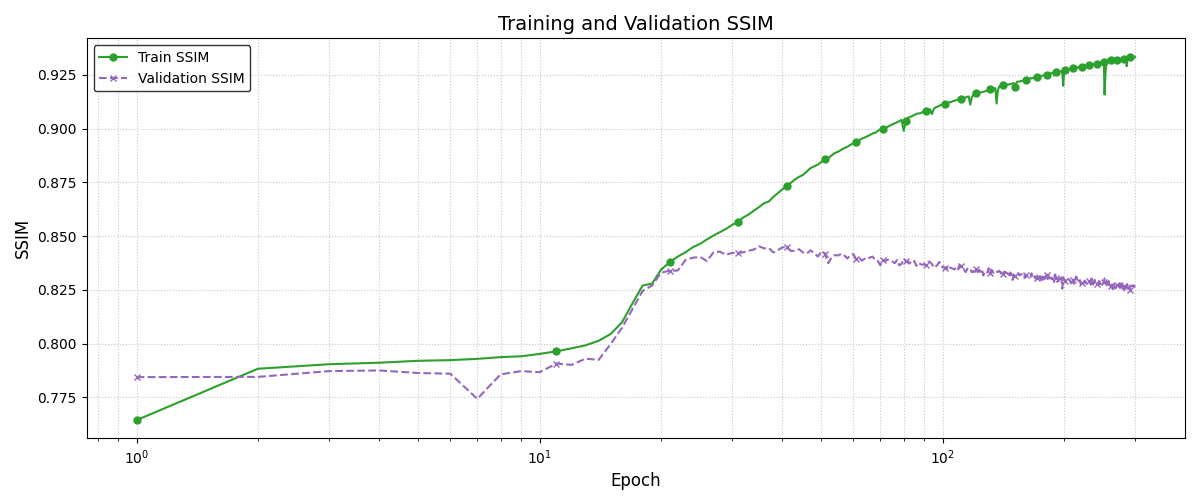
\includegraphics[width=0.7\linewidth]{images/colab_ssim_curve.png}
    \newline
    \small SSIM curve 
\end{frame}

\begin{frame}{Colab Training - Vectorial data vs Directional data}
    \begin{columns}
        \column{0.5\textwidth}
            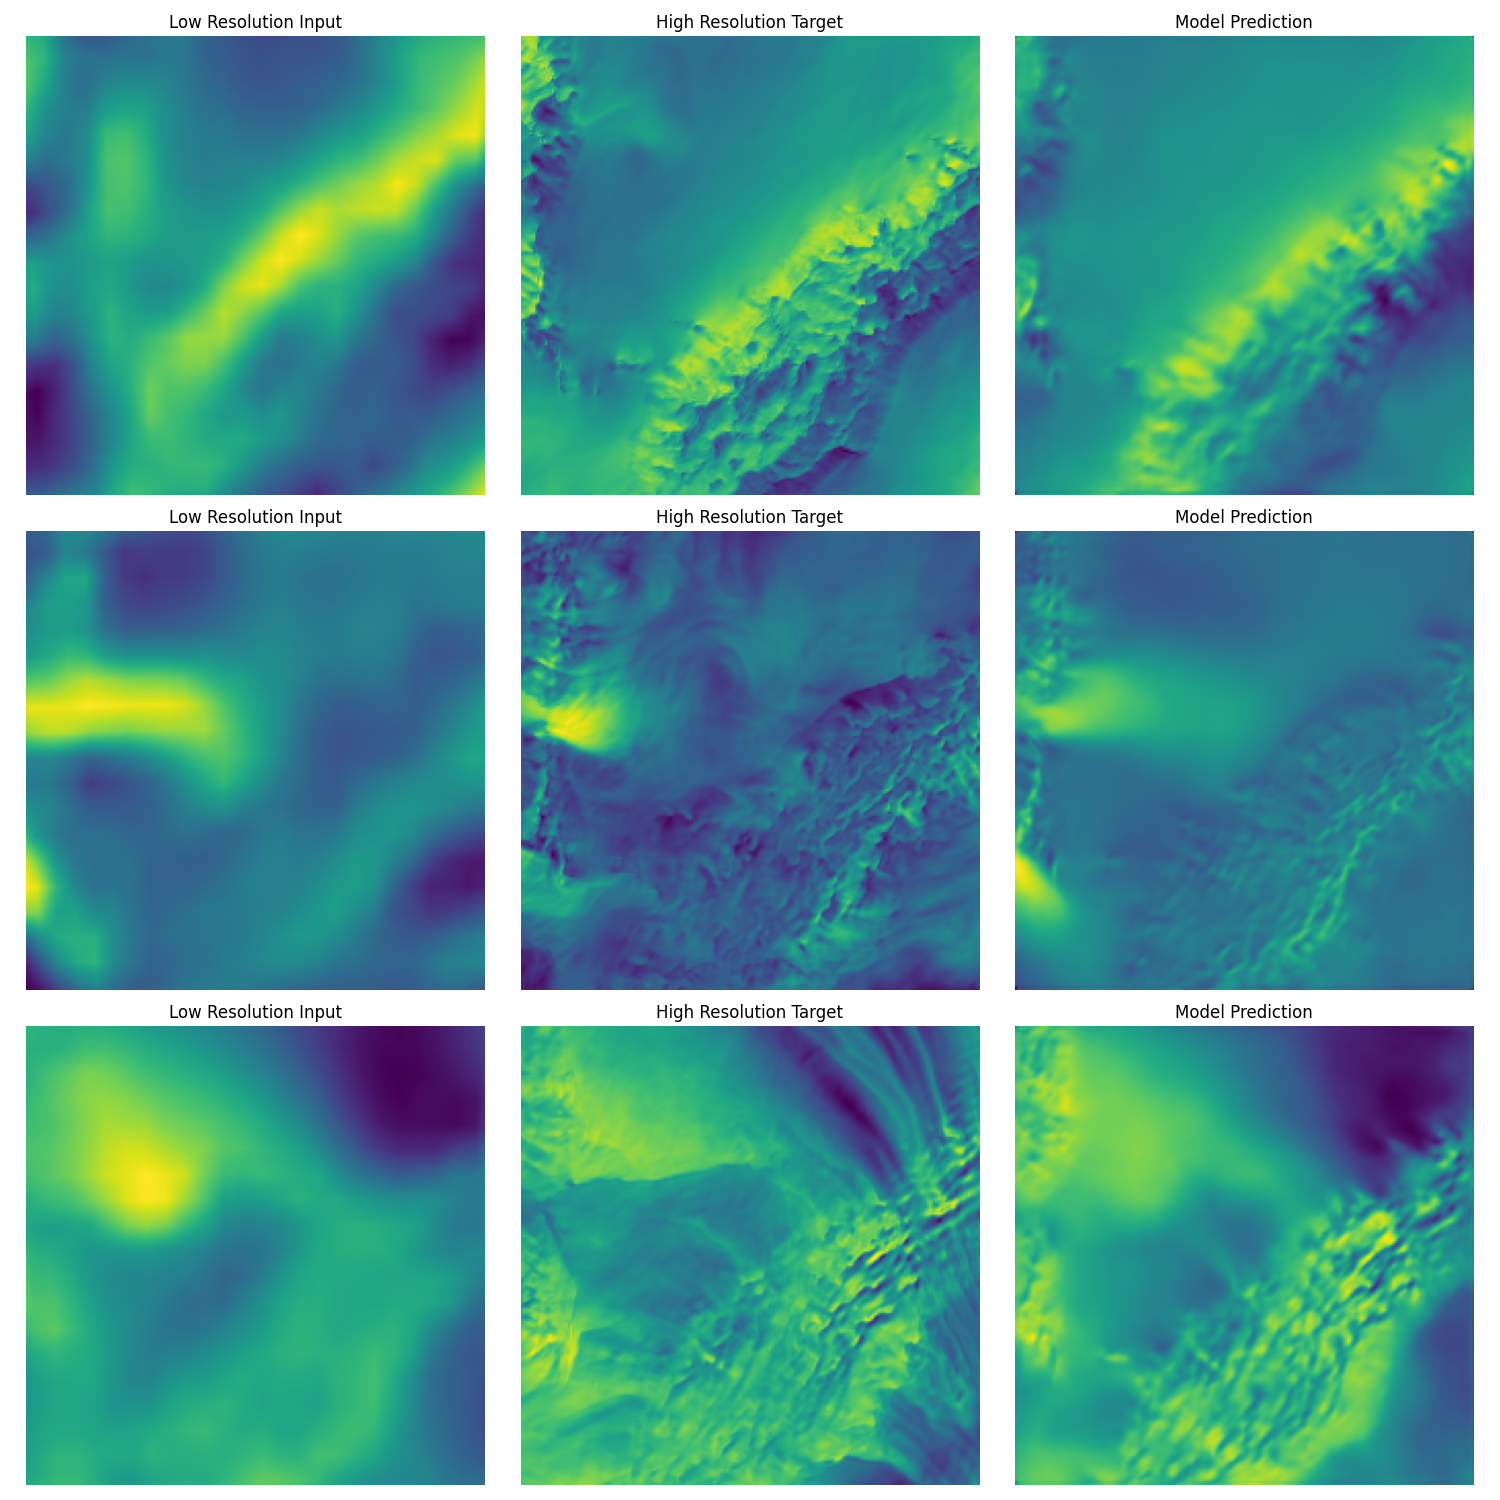
\includegraphics[width=\linewidth]{images/colab_vector_unet_L1SSIM_loss_300_epochs_8_batch_1em3_lr_1em5_weightdecay_best.pt.png}
            \newline
            \centering \small Vector data. SSIM: \texttt{0.84483}
        \column{0.5\textwidth}
            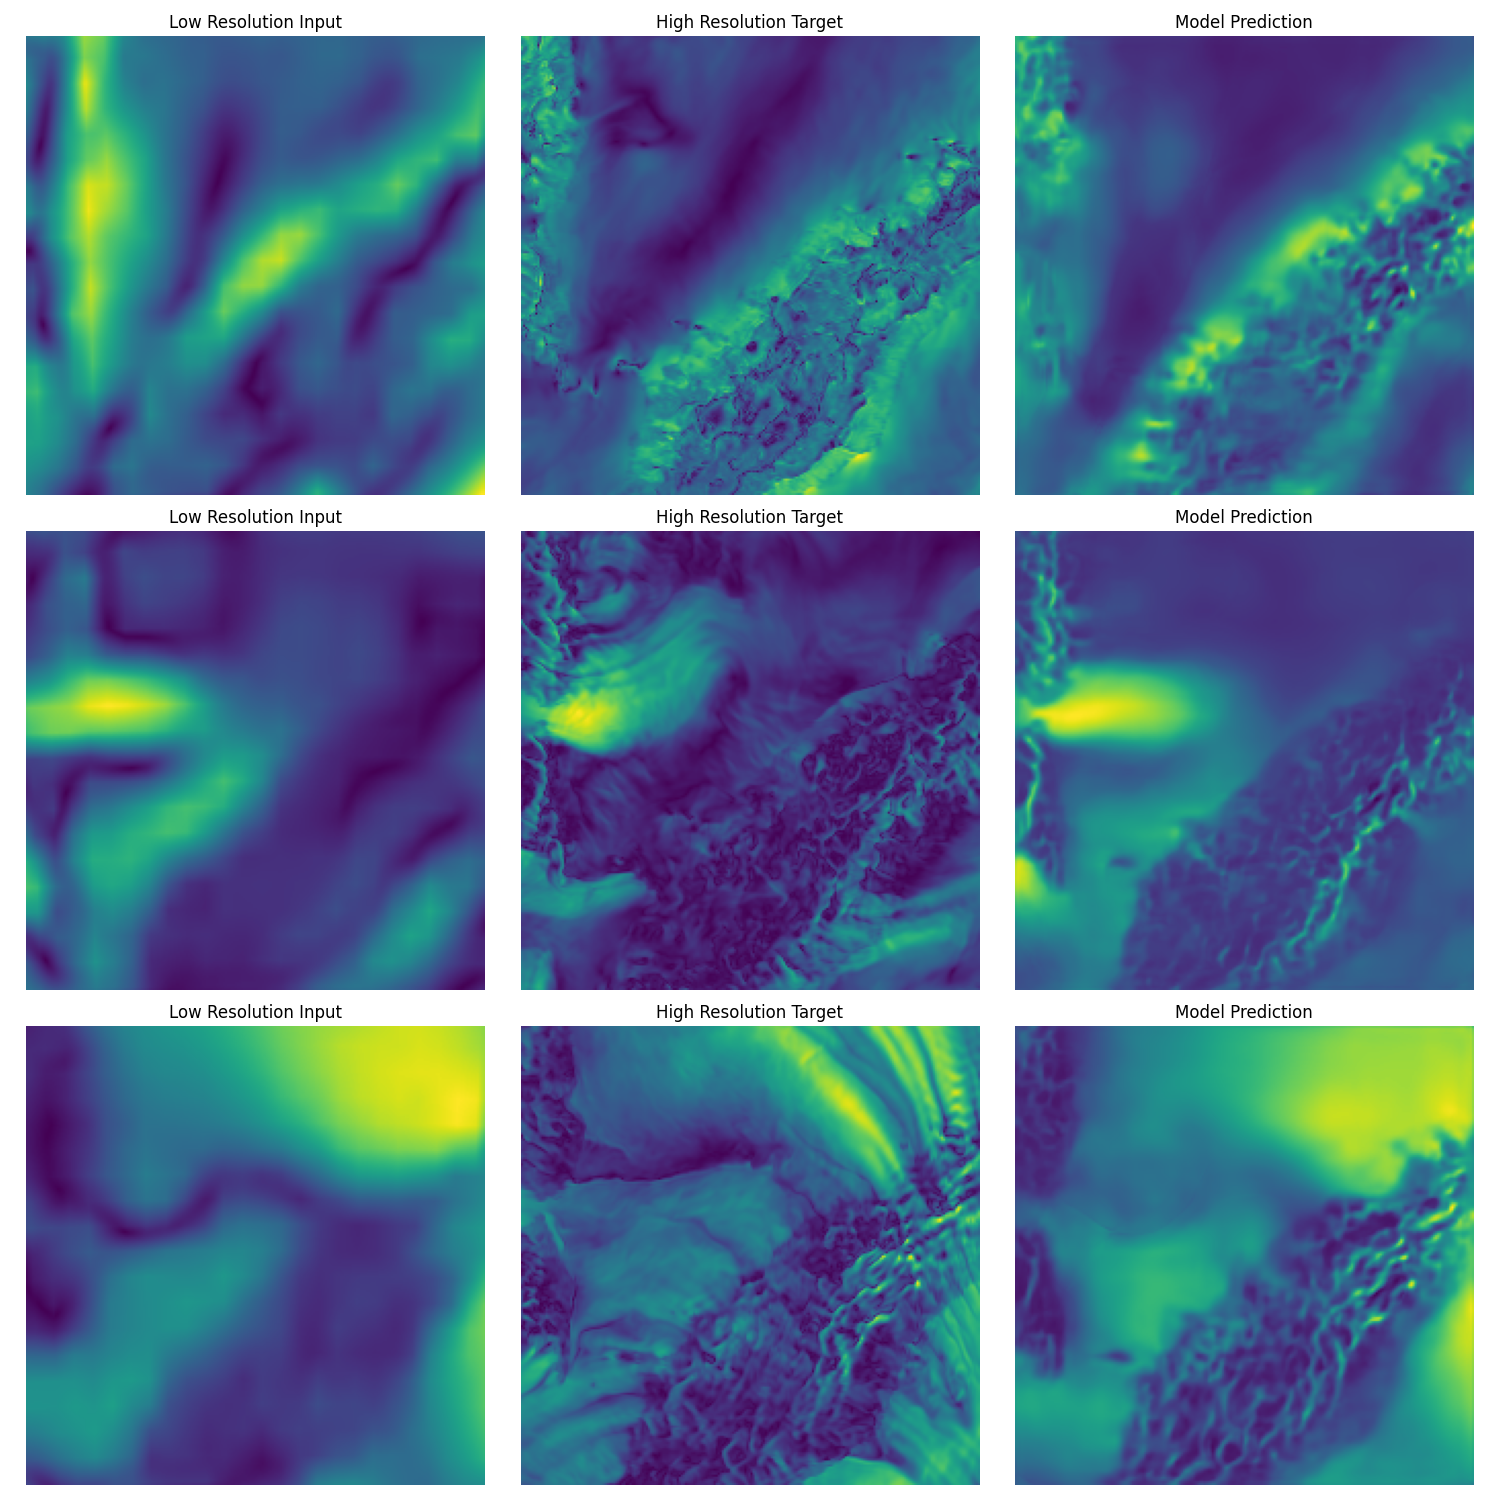
\includegraphics[width=\linewidth]{images/colab_direction_unet_L1SSIM_loss_150_epochs_4_batch_1em3_lr_1em5_weightdecay_best.pt.png}
            \newline
            \centering \small Direction data. SSIM: \texttt{0.48154}
    \end{columns}
\end{frame}
% FEDE
\begin{frame}{Results}
% mostrare i risultati finali per entrambi + un commento sulla differenza tra training locale con 100 immagini e training su colab con 1000
\end{frame}

% MARZIA
\begin{frame}{Final Considerations}
  \begin{itemize}
    \item Expectation: One representation may yield lower MSE and better visual fidelity.
    \item Trade-offs:
      \begin{itemize}
        \item Cartesian: linear inputs, but directional discontinuities.
        \item Polar: continuous angular information, but non-linear mapping.
      \end{itemize}
    \item Implications: Guidance for future climate data downscaling pipelines.
    \item Next steps:
      \begin{itemize}
        \item Extend to multilevel atmospheric variables.
        \item Evaluate on different regions and seasons.
      \end{itemize}
  \end{itemize}
\end{frame}
% come ci aspettavamo la rappresentazione con vettori e' quella migliore e quella con intensita' e direzione fa schifo al cazzo

\begin{frame}
    \frametitle{References}
    \printbibliography
\end{frame}
\end{document}

